\documentclass[tikz, border = 5pt]{standalone}

\begin{document}
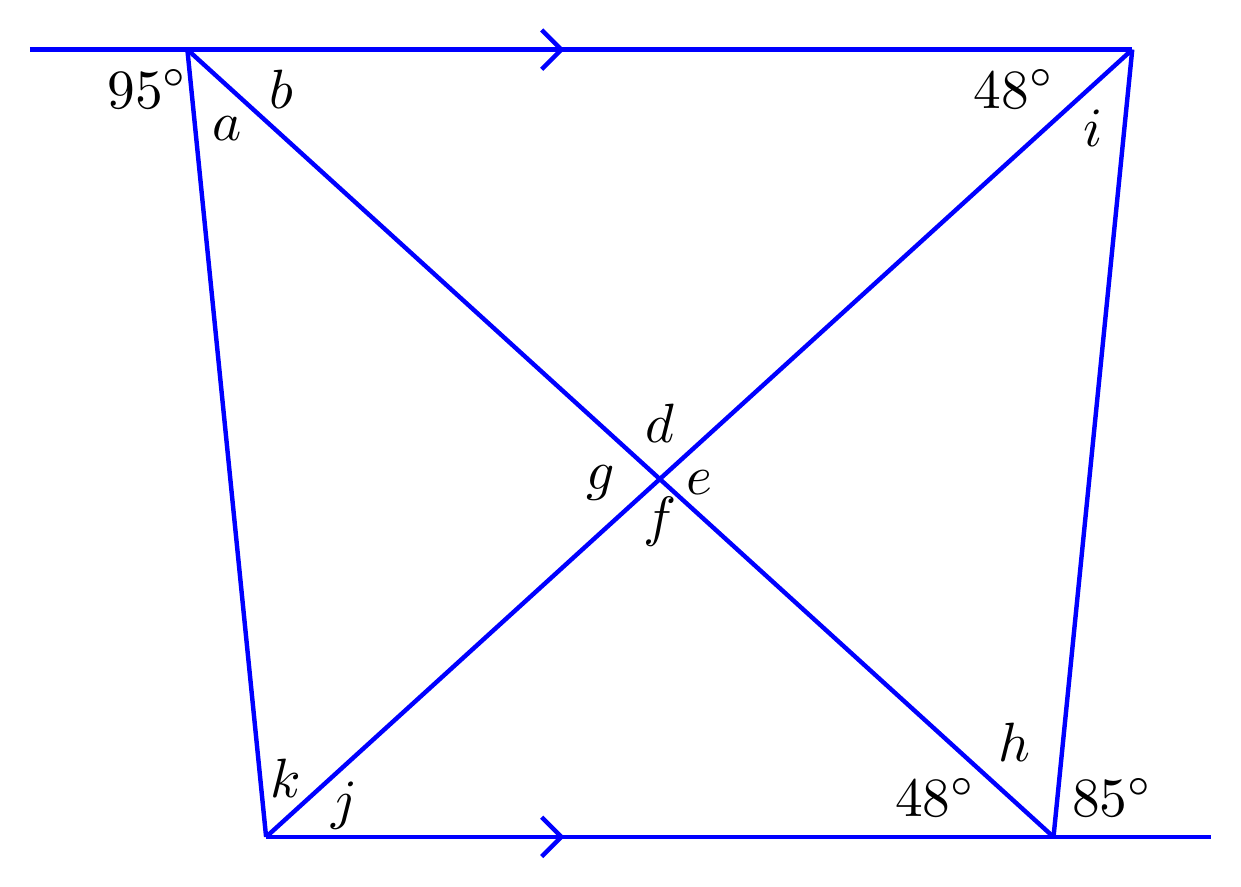
\begin{tikzpicture}

% grid
%\draw[help lines, step = 1cm] (0, 0) grid (15, 10);

\draw[ultra thick, smooth,blue, -] (0,10) -- (14,10);
\draw[ultra thick, smooth,blue, -] (2,10) -- (13,0);
\draw[ultra thick, smooth,blue, -] (2,10) -- (3,0);
\draw[ultra thick, smooth,blue, -] (3,0) -- (14,10);
\draw[ultra thick, smooth,blue, -] (3,0) -- (15,0);
\draw[ultra thick, smooth,blue, -] (13,0) -- (14,10);

% Arrows
\draw[ultra thick, smooth,blue, -] (6.5,10.25) -- (6.75,10);
\draw[ultra thick, smooth,blue, -] (6.5,9.75) -- (6.75,10);

\draw[ultra thick, smooth,blue, -] (6.5,0.25) -- (6.75,0);
\draw[ultra thick, smooth,blue, -] (6.5,-0.25) -- (6.75,0);

% labels
\node[scale=2] at (1.5,9.5) {$95^{\circ}$};
\node[scale=2] at (11.5,0.5) {$48^{\circ}$};
\node[scale=2] at (12.5,9.5) {$48^{\circ}$};
\node[scale=2] at (13.75,0.5) {$85^{\circ}$};
\node[scale=2] at (2.5,9) {$a$};
\node[scale=2] at (3.2,9.5) {$b$};
\node[scale=2] at (8,5.25) {$d$};
\node[scale=2] at (8.5,4.5) {$e$};
\node[scale=2] at (8,4) {$f$};
\node[scale=2] at (7.25,4.5) {$g$};
\node[scale=2] at (12.5,1.2) {$h$};
\node[scale=2] at (13.5,9) {$i$};
\node[scale=2] at (4,0.4) {$j$};
\node[scale=2] at (3.25,0.75) {$k$};

\end{tikzpicture}
\end{document}
